%%%%%%%%%%%%%%%%%%%%%%%%%%%%%%%%%%%%%%%%%
% Beamer Presentation
% LaTeX Template
% Version 1.0 (10/11/12)
%
% This template has been downloaded from:
% http://www.LaTeXTemplates.com
%
% License:
% CC BY-NC-SA 3.0 (http://creativecommons.org/licenses/by-nc-sa/3.0/)
%
%%%%%%%%%%%%%%%%%%%%%%%%%%%%%%%%%%%%%%%%%

%----------------------------------------------------------------------------------------
%	PACKAGES AND THEMES
%----------------------------------------------------------------------------------------

\documentclass{beamer}

\mode<presentation> {

% The Beamer class comes with a number of default slide themes
% which change the colors and layouts of slides. Below this is a list
% of all the themes, uncomment each in turn to see what they look like.

%\usetheme{default}
%\usetheme{AnnArbor}
%\usetheme{Antibes}
%\usetheme{Bergen}
%\usetheme{Berkeley}
%\usetheme{Berlin}
%\usetheme{Boadilla}
\usetheme{CambridgeUS}
%\usetheme{Copenhagen}
%\usetheme{Darmstadt}
%\usetheme{Dresden}
%\usetheme{Frankfurt}
%\usetheme{Goettingen}
%\usetheme{Hannover}
%\usetheme{Ilmenau}
%\usetheme{JuanLesPins}
%\usetheme{Luebeck}
%\usetheme{Madrid}
%\usetheme{Malmoe}
%\usetheme{Marburg}
%\usetheme{Montpellier}
%\usetheme{PaloAlto}
%\usetheme{Pittsburgh}
%\usetheme{Rochester}
%\usetheme{Singapore}
%\usetheme{Szeged}
%\usetheme{Warsaw}

% As well as themes, the Beamer class has a number of color themes
% for any slide theme. Uncomment each of these in turn to see how it
% changes the colors of your current slide theme.

%\usecolortheme{albatross}
%\usecolortheme{beaver}
%\usecolortheme{beetle}
%\usecolortheme{crane}
%\usecolortheme{dolphin}
%\usecolortheme{dove}
%\usecolortheme{fly}
%\usecolortheme{lily}
%\usecolortheme{orchid}
%\usecolortheme{rose}
%\usecolortheme{seagull}
%\usecolortheme{seahorse}
%\usecolortheme{whale}
%\usecolortheme{wolverine}

%\setbeamertemplate{footline} % To remove the footer line in all slides uncomment this line
\setbeamertemplate{footline}[page number] % To replace the footer line in all slides with a simple slide count uncomment this line

%\setbeamertemplate{navigation symbols}{} % To remove the navigation symbols from the bottom of all slides uncomment this line
}

\usepackage{graphicx} % Allows including images
\usepackage{booktabs} % Allows the use of \toprule, \midrule and \bottomrule in tables
\usepackage[utf8]{inputenc}
\usepackage[T1]{fontenc}
\usepackage[brazil]{babel}
\usepackage{amsmath}
\usepackage{amsfonts}
\usepackage{amssymb}
%----------------------------------------------------------------------------------------
%	TITLE PAGE
%----------------------------------------------------------------------------------------

\title[Tardes de Linguística]{Extração de Dados Linguísticos da Internet} % The short title appears at the bottom of every slide, the full title is only on the title page

\author{Bruno Guide e Beatriz Albiero} % Your name
\institute[USP] % Your institution as it will appear on the bottom of every slide, may be shorthand to save space
{
Grupo de Estudos de Linguística Computacional - Departamento de Linguística USP \\ % Your institution for the title page
\medskip
\textit{ling.compdl@gmail.com} % Your email address
}
\date{\today} % Date, can be changed to a custom date

\begin{document}

\begin{frame}
\titlepage % Print the title page as the first slide
\end{frame}

\begin{frame}
\frametitle{Índice} % Table of contents slide, comment this block out to remove it
\tableofcontents % Throughout your presentation, if you choose to use \section{} and \subsection{} commands, these will automatically be printed on this slide as an overview of your presentation
\end{frame}

%----------------------------------------------------------------------------------------
%	PRESENTATION SLIDES
%----------------------------------------------------------------------------------------
\section{Introdução}
%------------------------------------------------
\begin{frame}
\frametitle{Introdução}
\begin{itemize}
\item<1-> Popularização da computação  = Explosão de dados disponíveis.\\
\item<2-> Em específico, muitos dados na forma de língua escrita.\\
\item<3> Grande interesse em explorar esses dados de forma automatizada.\\
\end{itemize}
\end{frame}
%------------------------------------------------
\begin{frame}
\frametitle{Introdução}
\begin{itemize}
\item<1-> Esses dados podem ser úteis para a pesquisa linguística!\\
\item<2-> Importante ter em mente os possíveis problemas que isso pode causar.\\
\item<3> O que limita a extração automática?\\
\end{itemize}
\end{frame}
%------------------------------------------------

\section{Três problemas de coleta de dados} % Sections can be created in order to organize your presentation into discrete blocks, all sections and subsections are automatically printed in the table of contents as an overview of the talk
%------------------------------------------------

\begin{frame}
\frametitle{Três problemas de coleta de dados}
\begin{itemize}
\item Verbos Irregulares\\
\item Comparação entre línguas distintas\\
\item Palavras mais buscadas no site Dicio.com.br\\
\end{itemize}
\end{frame}

\subsection{Verbos Irregulares}
\begin{frame}
\frametitle{Verbos Irregulares}
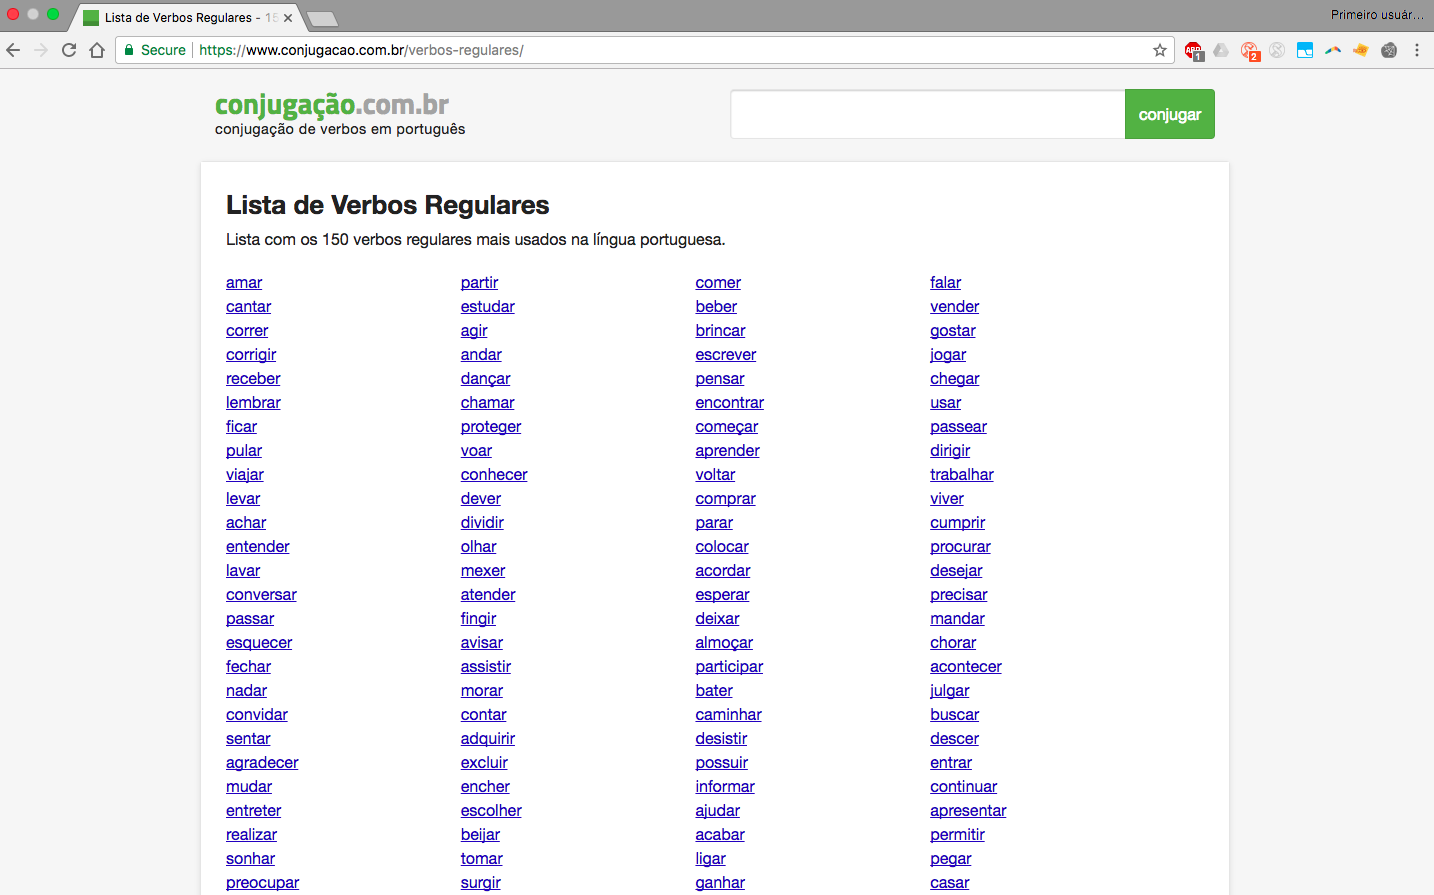
\includegraphics[width=\textwidth]{Screen_Shot_2017-10-05_at_21_21_15.png}
\end{frame}
%------------------------------------------------

\subsection{Comparação entre línguas distintas}
\begin{frame}
\frametitle{Coletando dados de línguas distintas}
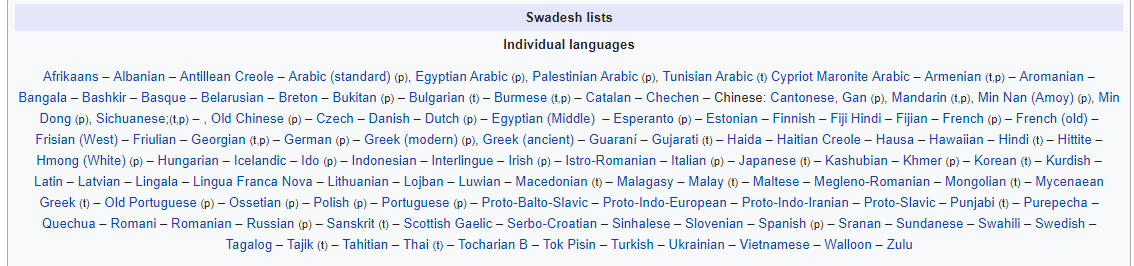
\includegraphics[width=\textwidth]{ListaDeQuadros.png}
\end{frame}

\begin{frame}
\frametitle{Coletando dados de línguas distintas}
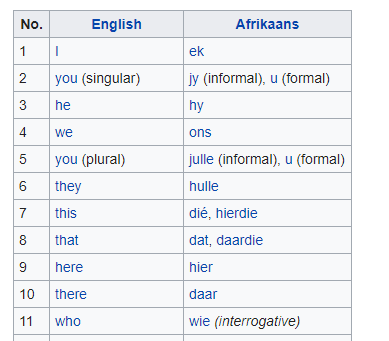
\includegraphics[width=\textwidth]{QuadroComparativo.png}
\end{frame}


\subsection{Palavras mais buscadas no site Dicio.com.br} 

\begin{frame}
\frametitle{Palavras mais buscadas no site Dicio.com.br}
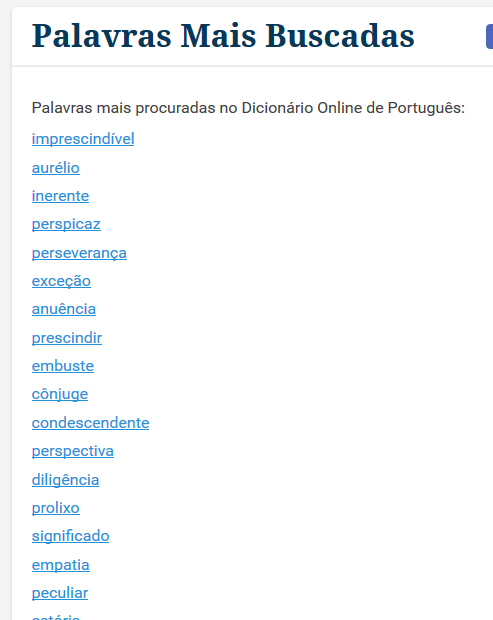
\includegraphics[width=\textwidth]{Dicio_com_br.png}
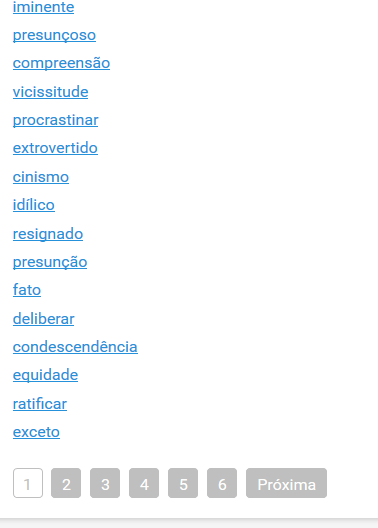
\includegraphics[width=\textwidth]{Dicio2_com_br.png}
\end{frame}



\section{Extração Automática}
%------------------------------------------------

\subsection{Dados Estruturados vs. Dados Não-Estruturados} 

%------------------------------------------------
\begin{frame}
\frametitle{Dados Estruturados vs. Dados Não-Estruturados}
\begin{itemize}
\item <1-> Automatização requer consistência e organização.\\
\item <2-> Os dados que são consistentes e organizados chamamos de \textit{estruturados}\\
\item <3-> Por outro lado temos os dados \textit{não-estruturados}.\\
\item <4> Essa questão é fundamental.\\
\end{itemize}
\end{frame}
%------------------------------------------------
\begin{frame}
\frametitle{Dados Estruturados vs. Dados Não-Estruturados}
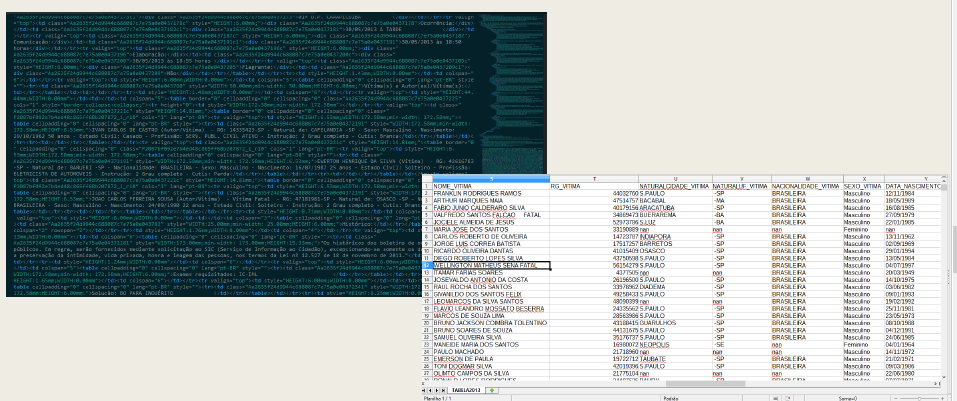
\includegraphics[width=\textwidth]{DadosEstr.png}
\end{frame}
%------------------------------------------------

\subsection{Web como fonte: Código Fonte e HTML} 
%------------------------------------------------
\begin{frame}
\frametitle{Web como fonte: A Web}
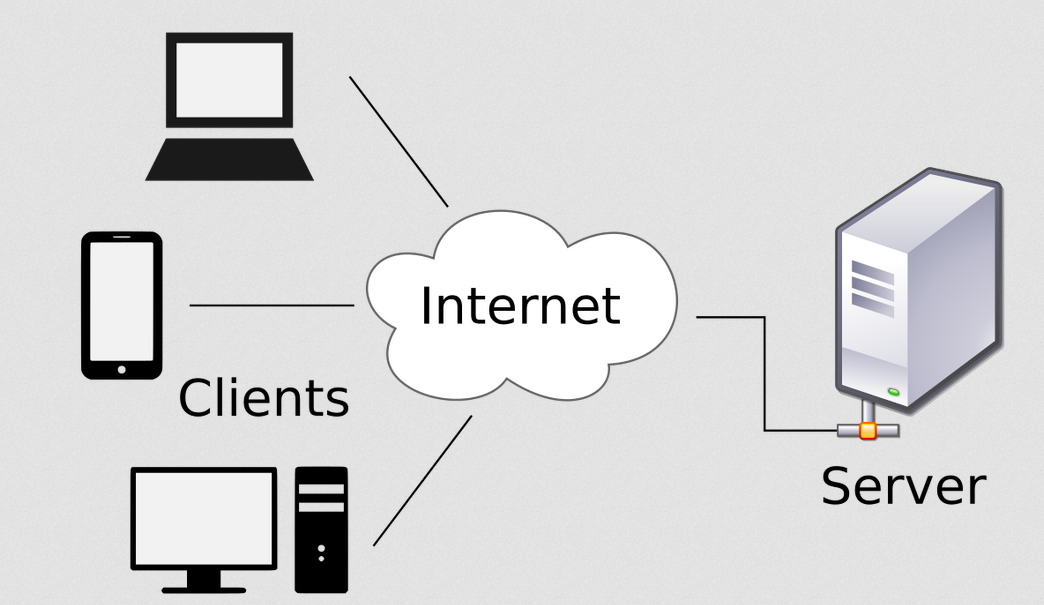
\includegraphics[width=\textwidth]{ClientServer.png}
\end{frame}
%------------------------------------------------
\begin{frame}
\frametitle{Web como fonte: Código Fonte e HTML}
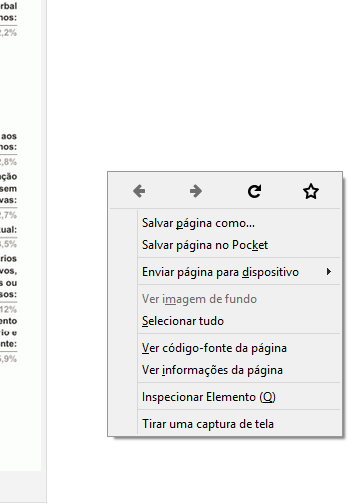
\includegraphics[width=.3\textwidth]{CodigoFonte.png}%
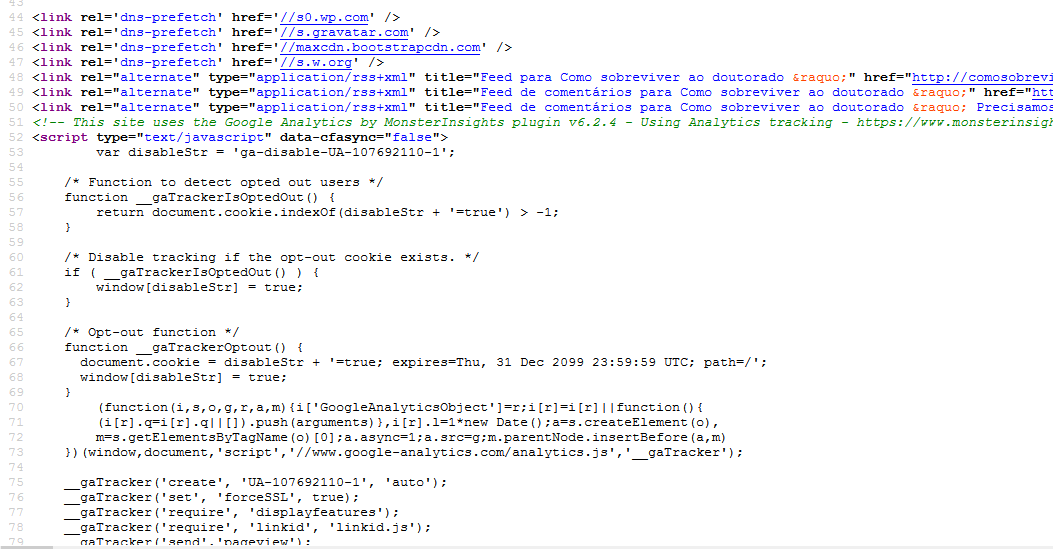
\includegraphics[width=.7\textwidth]{HtmlExemplo.png}
\end{frame}

\subsection{Reconhecendo Padrões e Tabulando dados}

%------------------------------------------------
\begin{frame}
\frametitle{Reconhecendo Padrões em HMTL}
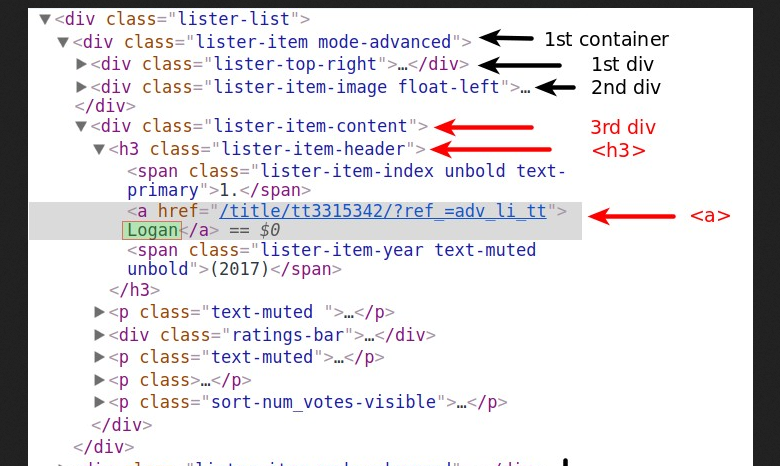
\includegraphics[width=\textwidth]{NestedTags.png}
\end{frame}
%------------------------------------------------
\begin{frame}
\frametitle{Tabulando dados}
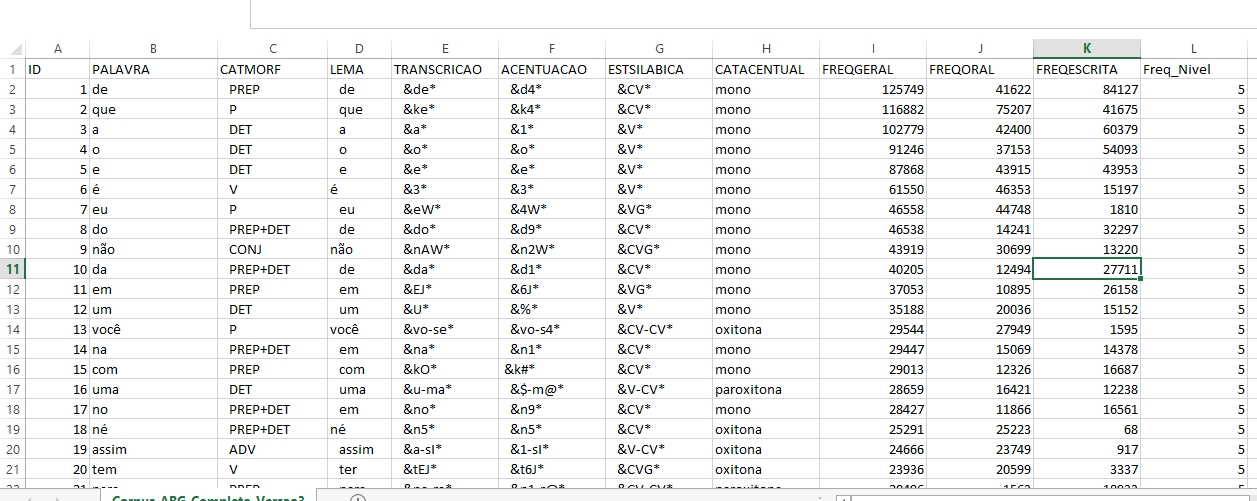
\includegraphics[width=\textwidth]{DadosTabulados.png}
\end{frame}

%------------------------------------------------
\begin{frame}
\frametitle{Processando dados}
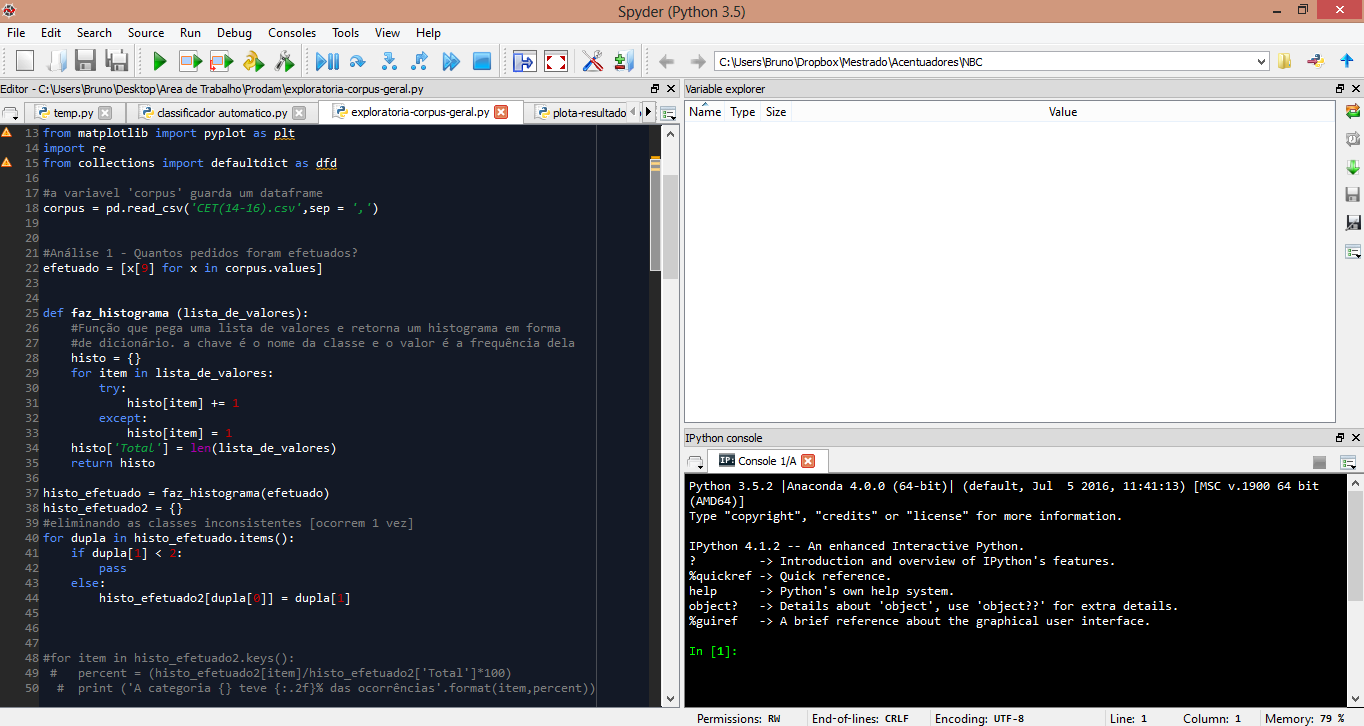
\includegraphics[width=\textwidth]{spyder.png}
\end{frame}

%------------------------------------------------
\section{Webscraper e Scrapy/BeautifulSoup}
%------------------------------------------------

\subsection{Webscraper} % A subsection can be created just before a set of slides with a common theme to further break down your presentation into chunks
\begin{frame}
\frametitle{Webscraper}
\begin{itemize}
\item Extensão do chrome para baixar automaticamente dados.\\
\item Possui interface intuitiva.\\
\item Não precisa passar da lógica visual para a do HTML!\\
\end{itemize}
\end{frame}

\subsection{Instalação e Tutoriais} % A subsection can be created just before a set of slides with a common theme to further break down your presentation into chunks

%------------------------------------------------

\begin{frame}
\frametitle{Instalação Webscraper}
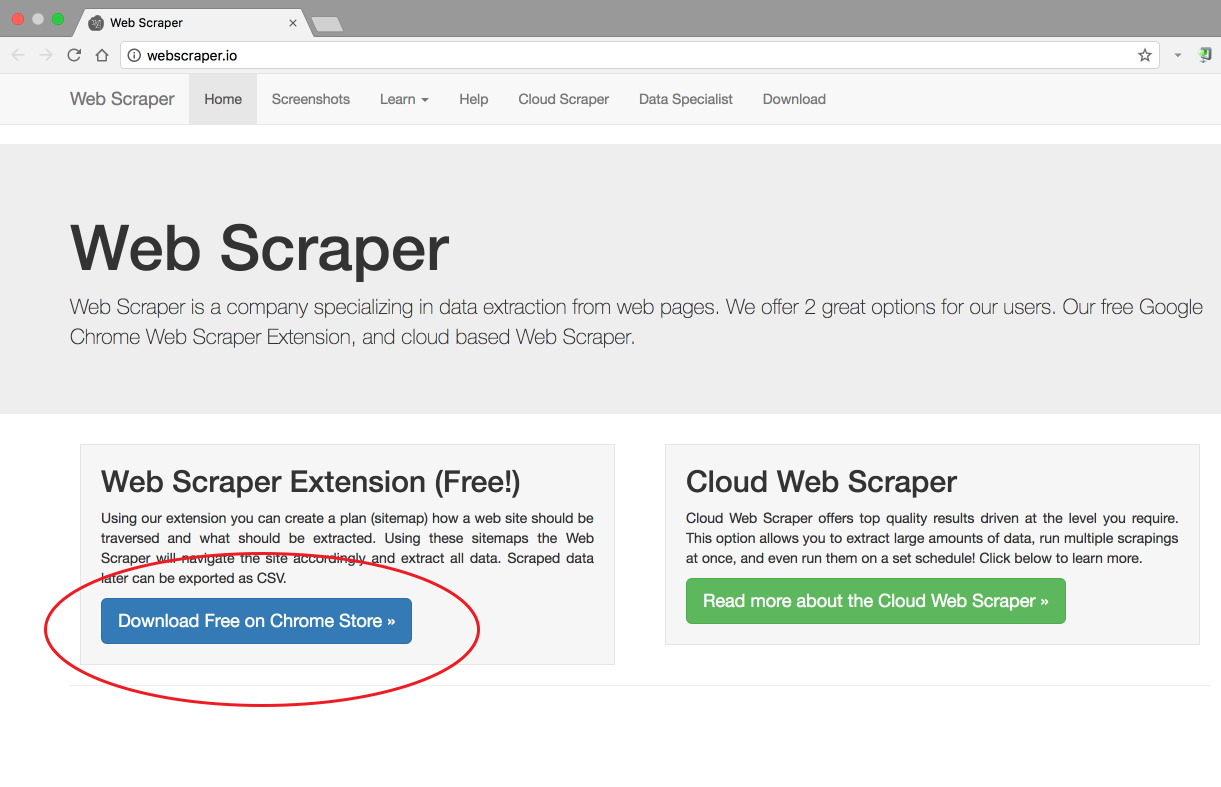
\includegraphics[width=\textwidth]{WhatsApp_Image_2017-10-05_at_17_22_43.jpg}
\end{frame}

%------------------------------------------------
\begin{frame}
\frametitle{Instalação Webscraper}
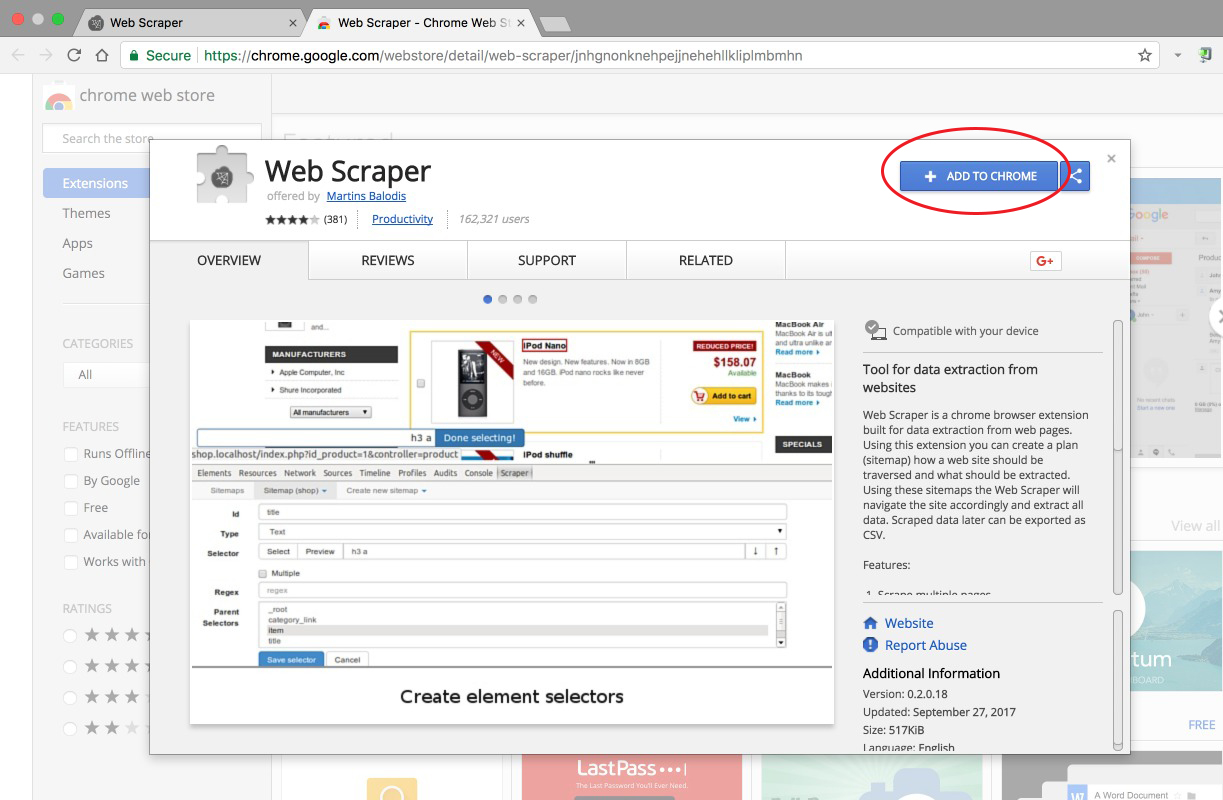
\includegraphics[width=\textwidth]{WhatsApp_Image_2017-10-05_at_17_22_44.jpg}
\end{frame}

%------------------------------------------------
\begin{frame}
\frametitle{Instalação Webscraper}
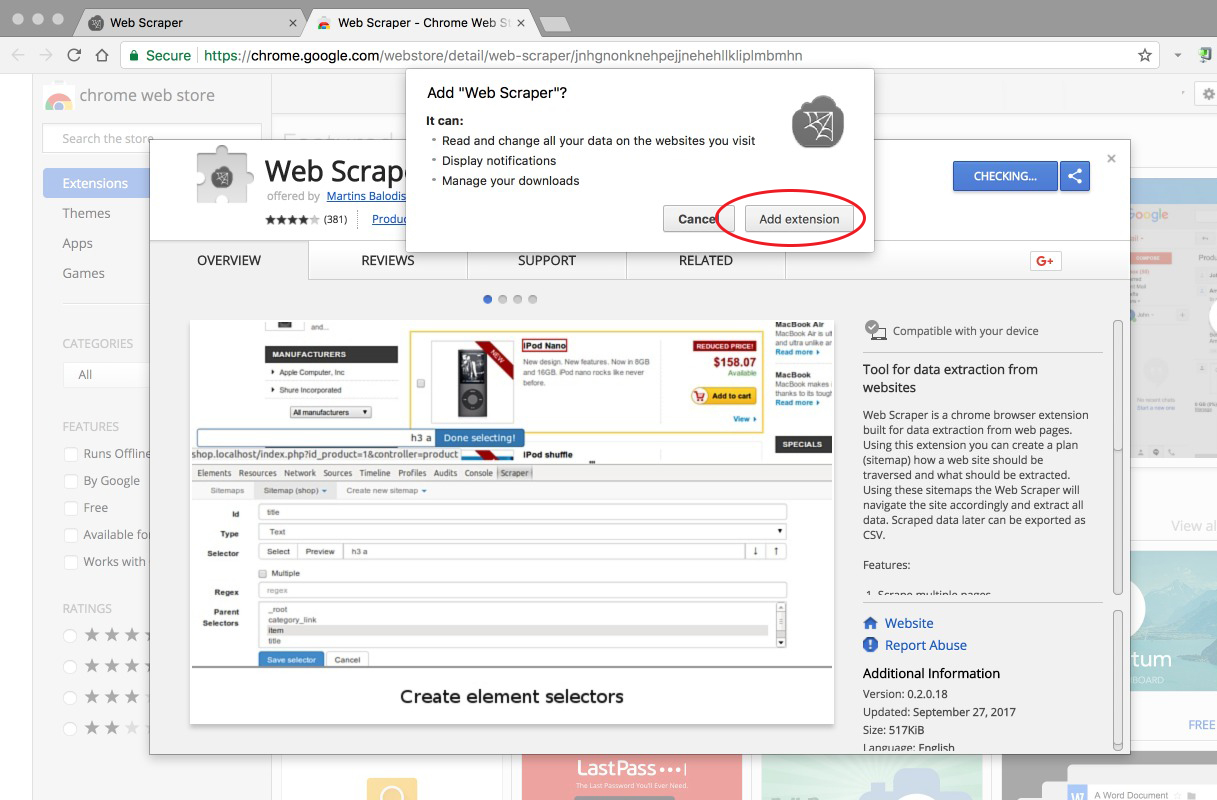
\includegraphics[width=\textwidth]{WhatsApp_Image_2017-10-05_at_17_22_44__1_.jpg}
\end{frame}

%------------------------------------------------
\begin{frame}
\frametitle{Instalação Webscraper}
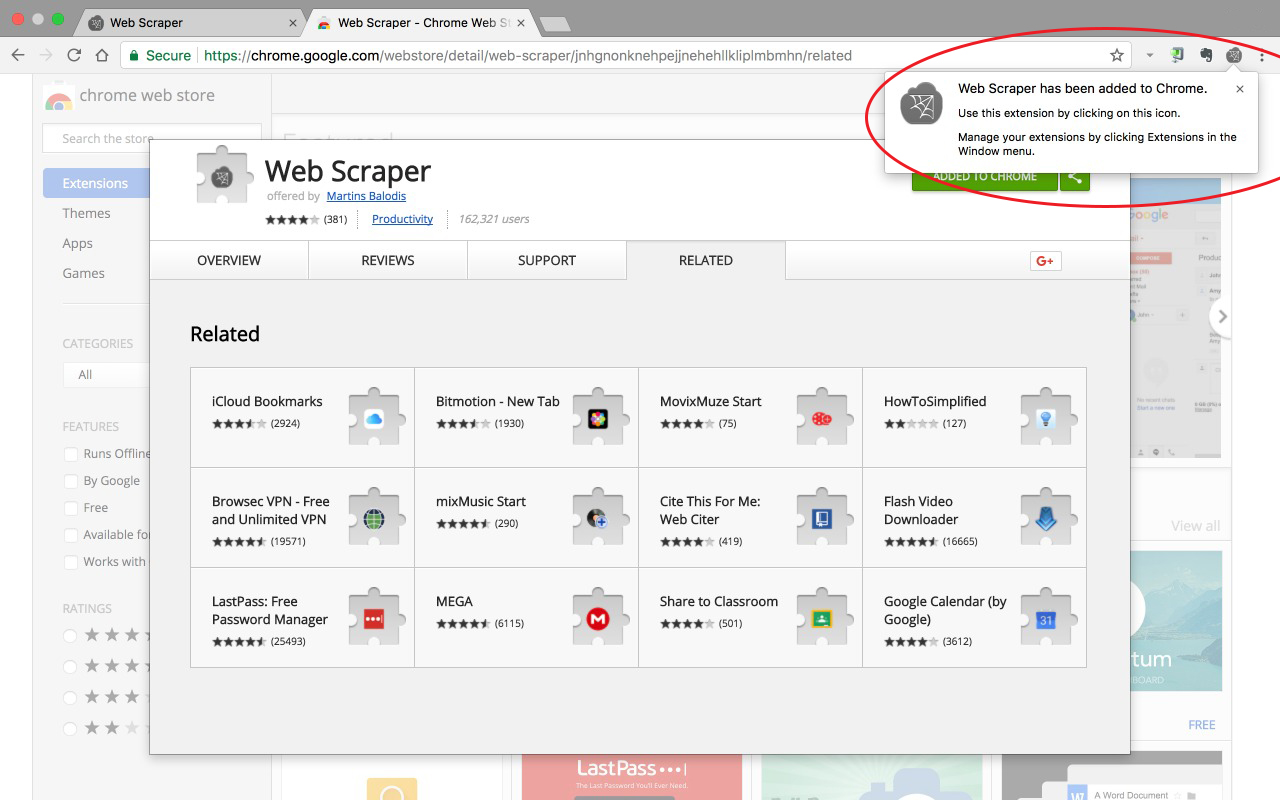
\includegraphics[width=\textwidth]{WhatsApp_Image_2017-10-05_at_17_22_44__2_.jpg}
\end{frame}


\subsection{Alternativa: Scrapy/BeautifulSoup (Prós e Contras)} %------------------------------------------------
\begin{frame}
\frametitle{Scrapy: uma alternativa}
\begin{itemize}
\item Bibliotecas Python para extração automática de dados Web.\\
\item Site: https://scrapy.org/ e  https://www.crummy.com/software/BeautifulSoup/bs4/doc/\\
\item Livro ensinando a usar.\\
\end{itemize}
\end{frame}
%------------------------------------------------
\begin{frame}
\frametitle{Scrapy: Prós e Contras}
\begin{itemize}
\item[(+)] Ferramenta muito poderosa. Automatiza coletas de dados extremamente complexas.\\
\item[(+)] Muito veloz. Bom para grandes quantidades de dados.\\
\item[( - )] Exige mais familiaridade com programação.\\
\item[( - )] Exige traduzir a lógica visual em lógica HTML.\\
\end{itemize}
\end{frame}

%------------------------------------------------
\section{Problemas Resolvidos}
%------------------------------------------------
\begin{frame}
\frametitle{Exemplo - Verbos}
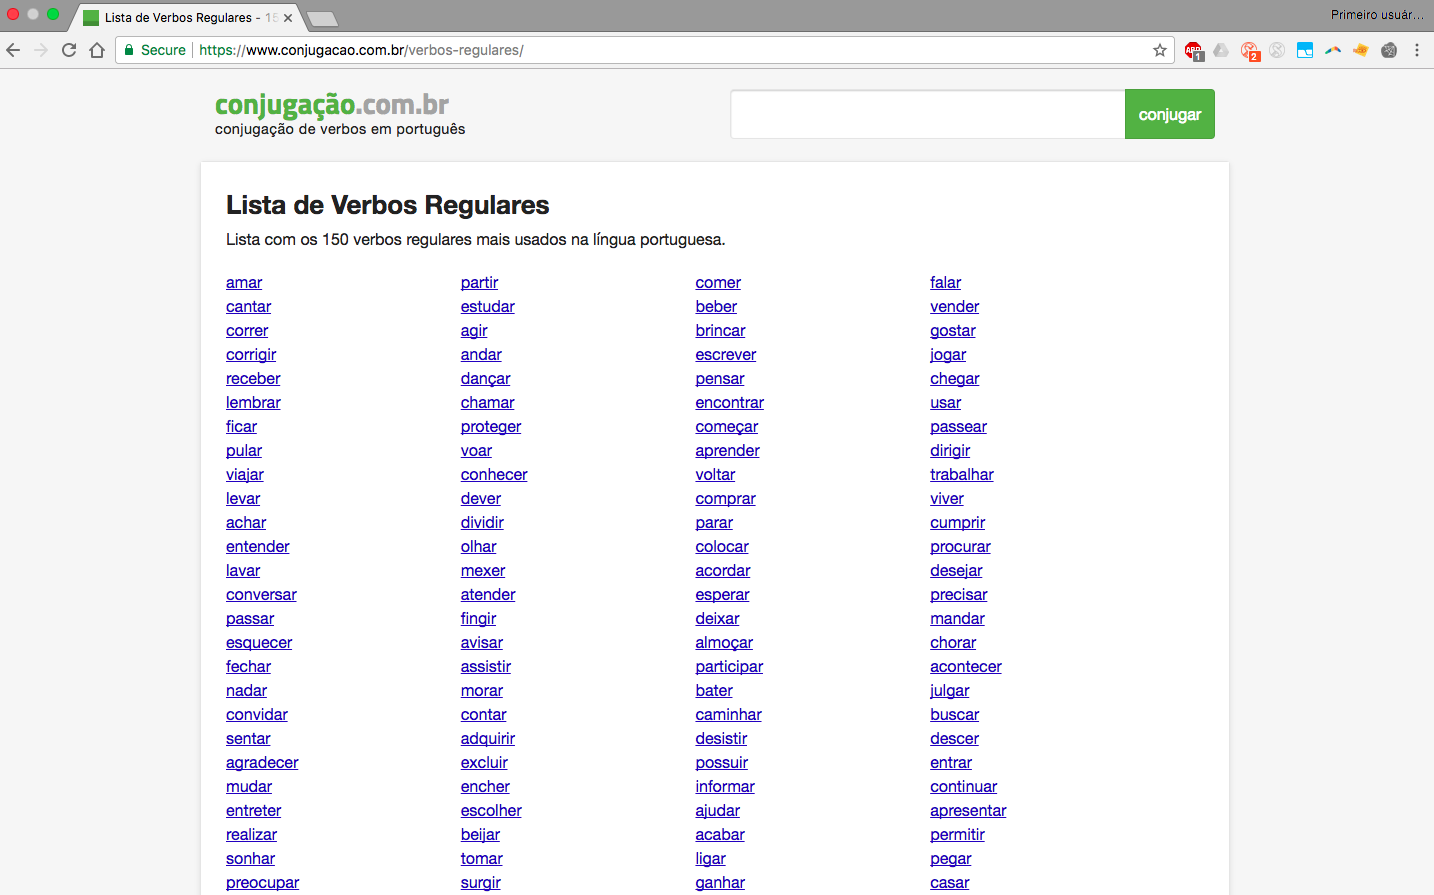
\includegraphics[width=\textwidth]{Screen_Shot_2017-10-05_at_21_21_15.png}
\end{frame}
%------------------------------------------------
\begin{frame}
\frametitle{Exemplo - Verbos}
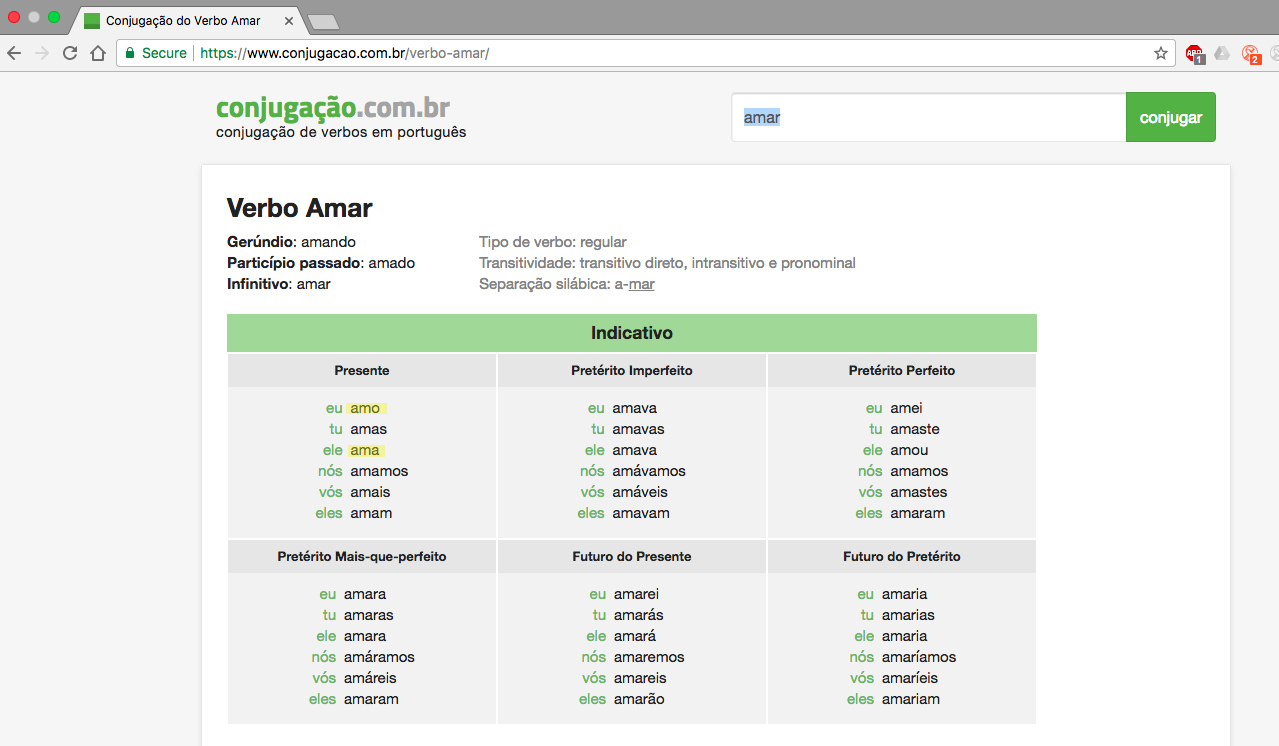
\includegraphics[width=\textwidth]{Screen_Shot_2017-10-05_at_21_26_26.jpg}
\end{frame}

%------------------------------------------------
\begin{frame}
\frametitle{Exemplo - Verbos}
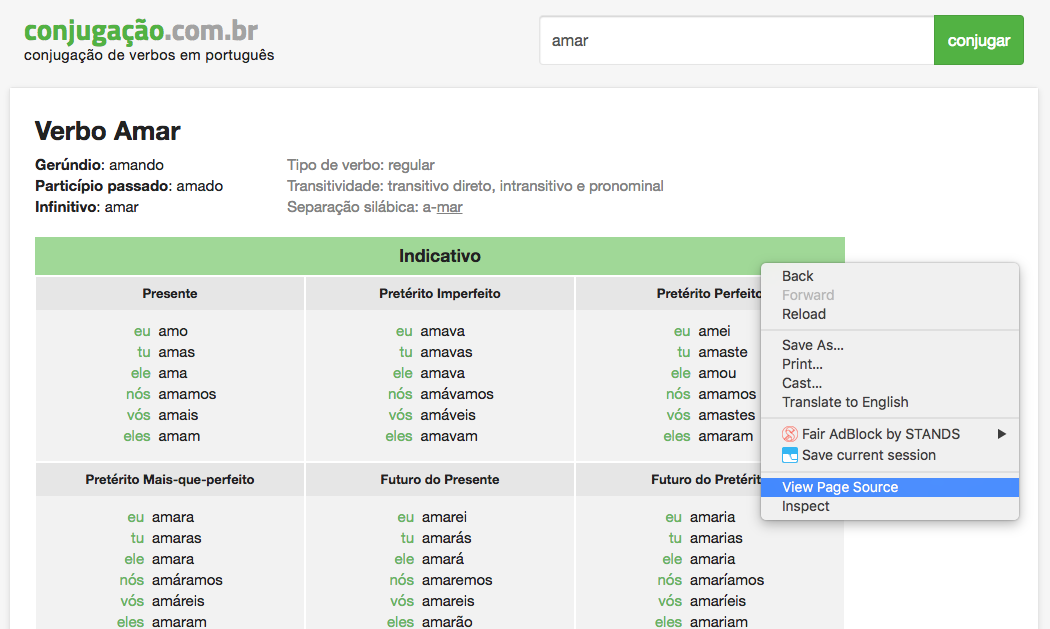
\includegraphics[width=\textwidth]{Screen_Shot_2017-10-05_at_22_12_00.png}
\end{frame}

%------------------------------------------------
\begin{frame}
\frametitle{Exemplo - Verbos}
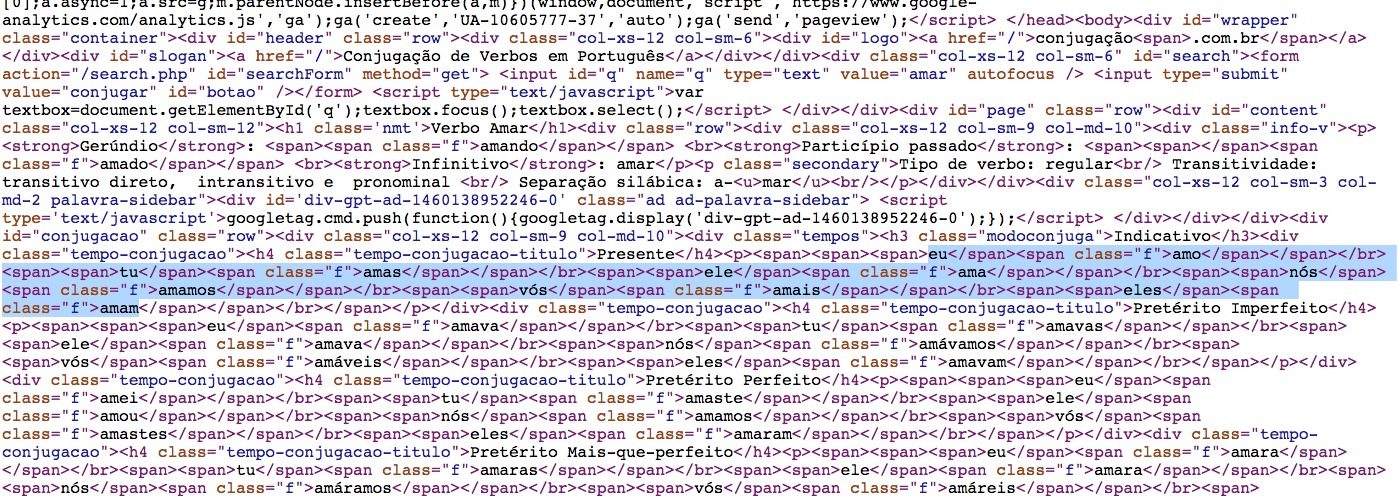
\includegraphics[width=\textwidth]{Screen_Shot_2017-10-05_at_22_17_35.png}
\end{frame}

%------------------------------------------------
\begin{frame}
\frametitle{Exemplo - Verbos}
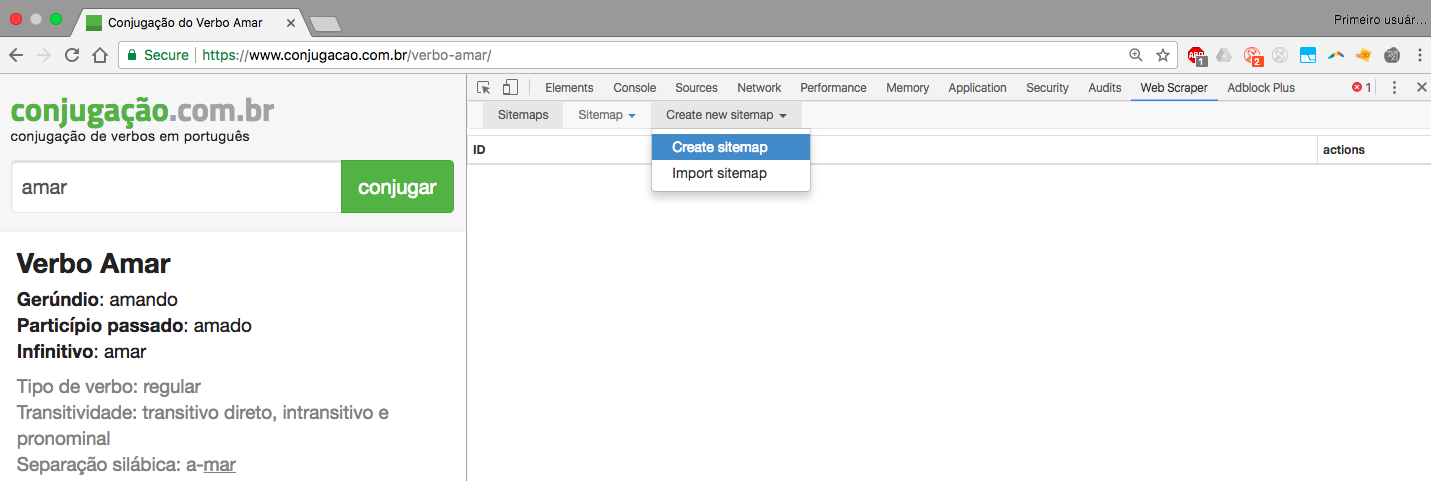
\includegraphics[width=\textwidth]{Screen_Shot_2017-10-05_at_22_22_43.png}
\end{frame}

%------------------------------------------------
\begin{frame}
\frametitle{Exemplo - Verbos}
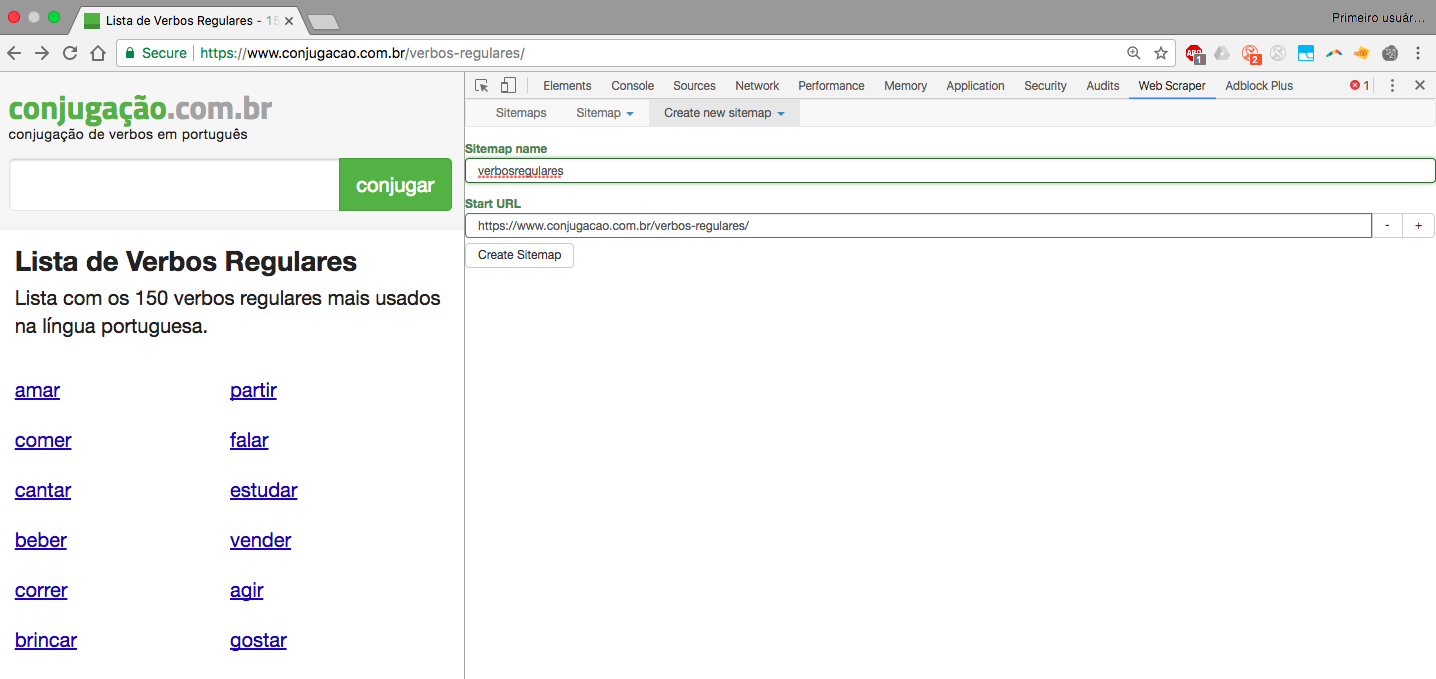
\includegraphics[width=\textwidth]{Screen_Shot_2017-10-05_at_22_23_21.png}
\end{frame}

%------------------------------------------------
\begin{frame}
\frametitle{Exemplo - Verbos}
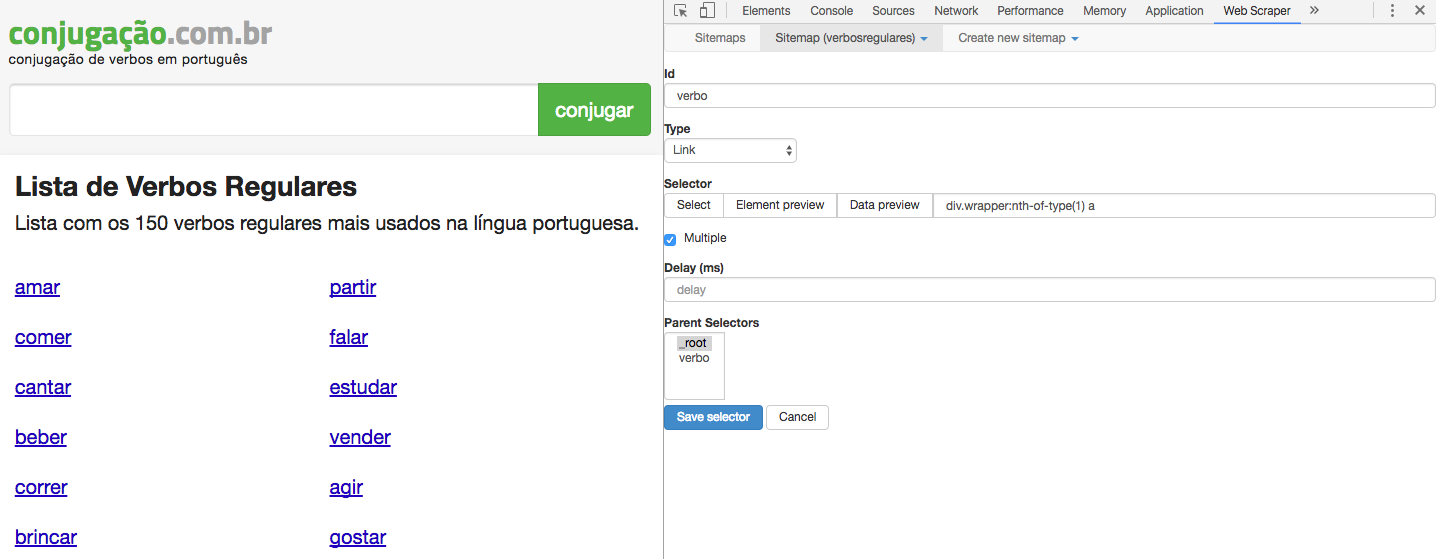
\includegraphics[width=\textwidth]{Screen_Shot_2017-10-05_at_22_47_52.png}
\end{frame}

%------------------------------------------------
\begin{frame}
\frametitle{Exemplo - Verbos}
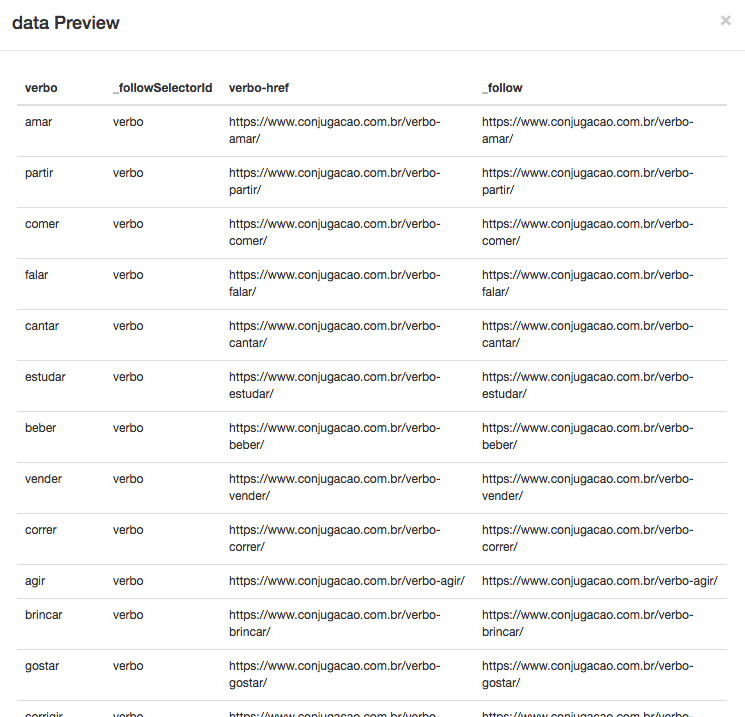
\includegraphics[width=\textwidth]{Screen_Shot_2017-10-05_at_22_49_47.png}
\end{frame}

%------------------------------------------------
\begin{frame}
\frametitle{Exemplo - Verbos}
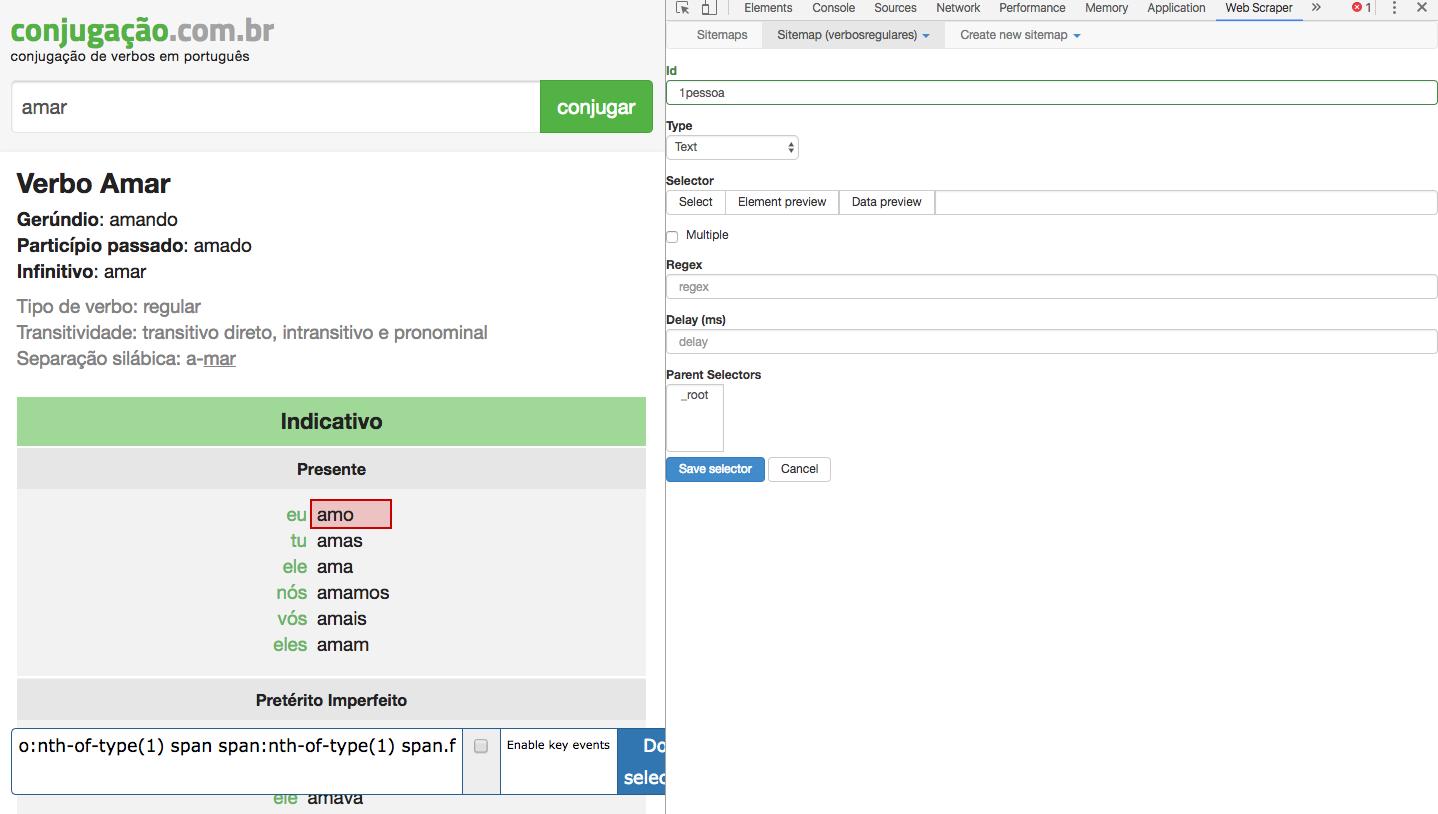
\includegraphics[width=\textwidth]{Screen_Shot_2017-10-05_at_22_27_52.png}
\end{frame}

%------------------------------------------------
\begin{frame}
\frametitle{Exemplo - Verbos}
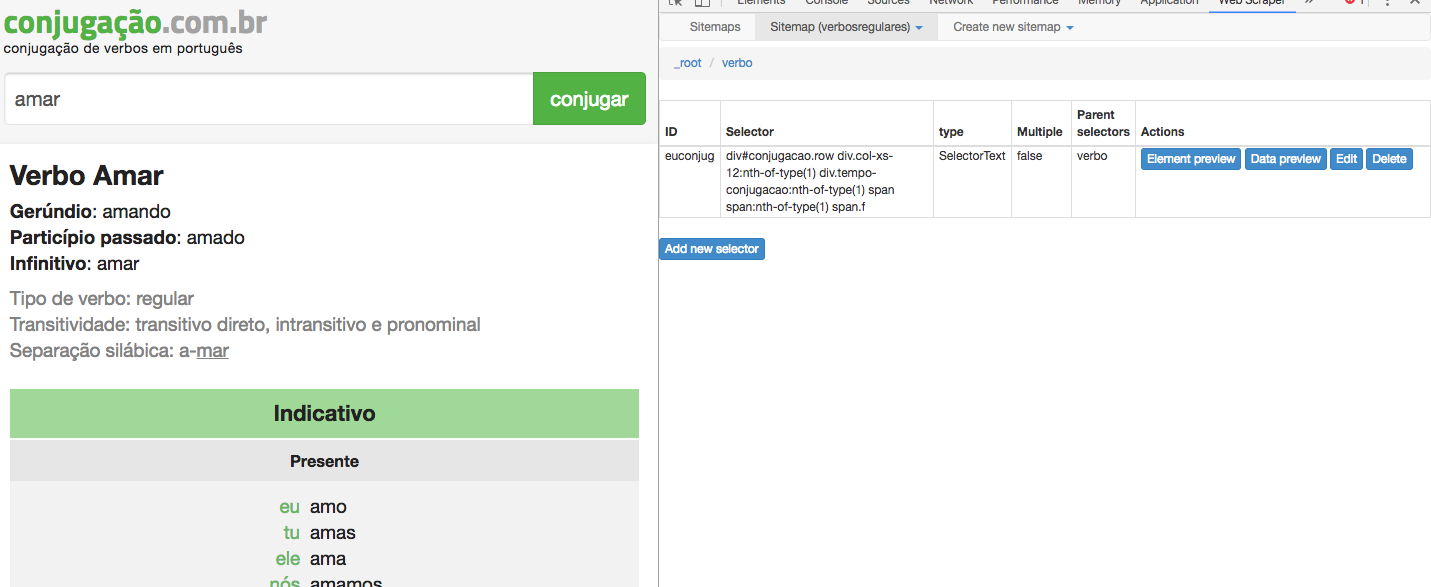
\includegraphics[width=\textwidth]{Screen_Shot_2017-10-05_at_22_42_33.png}
\end{frame}

%------------------------------------------------
\begin{frame}
\frametitle{Exemplo - Verbos}
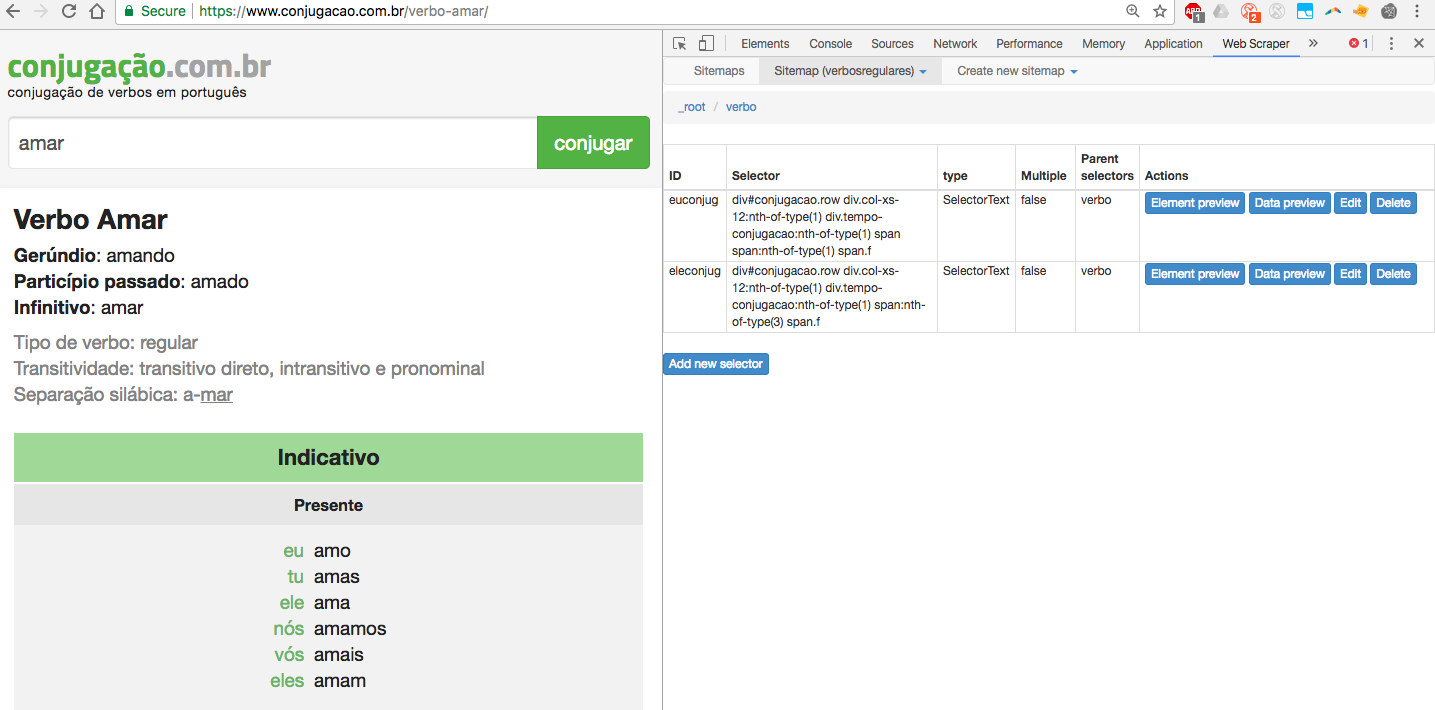
\includegraphics[width=\textwidth]{Screen_Shot_2017-10-05_at_22_43_03.png}
\end{frame}

%------------------------------------------------
\begin{frame}
\frametitle{Exemplo - Verbos}
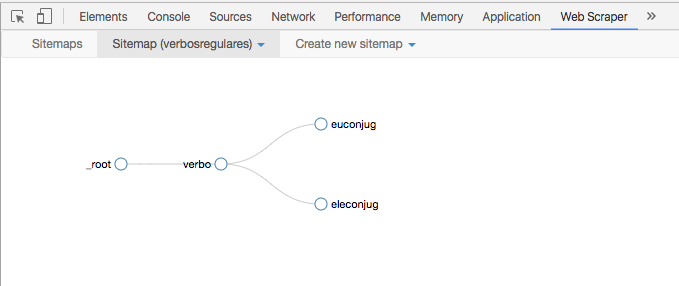
\includegraphics[width=\textwidth]{Screen_Shot_2017-10-05_at_22_43_19.png}
\end{frame}

%------------------------------------------------
\begin{frame}
\frametitle{Exemplo - Verbos}
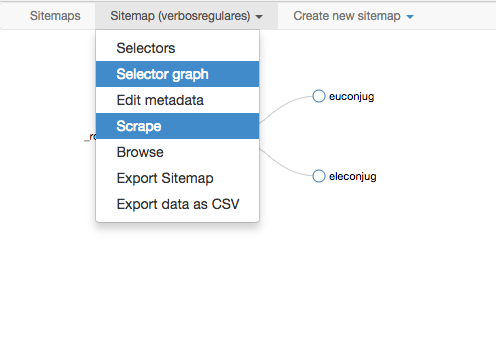
\includegraphics[width=\textwidth]{Screen_Shot_2017-10-05_at_22_54_07.png}
\end{frame}

%------------------------------------------------
\begin{frame}
\frametitle{Exemplo - Verbos}
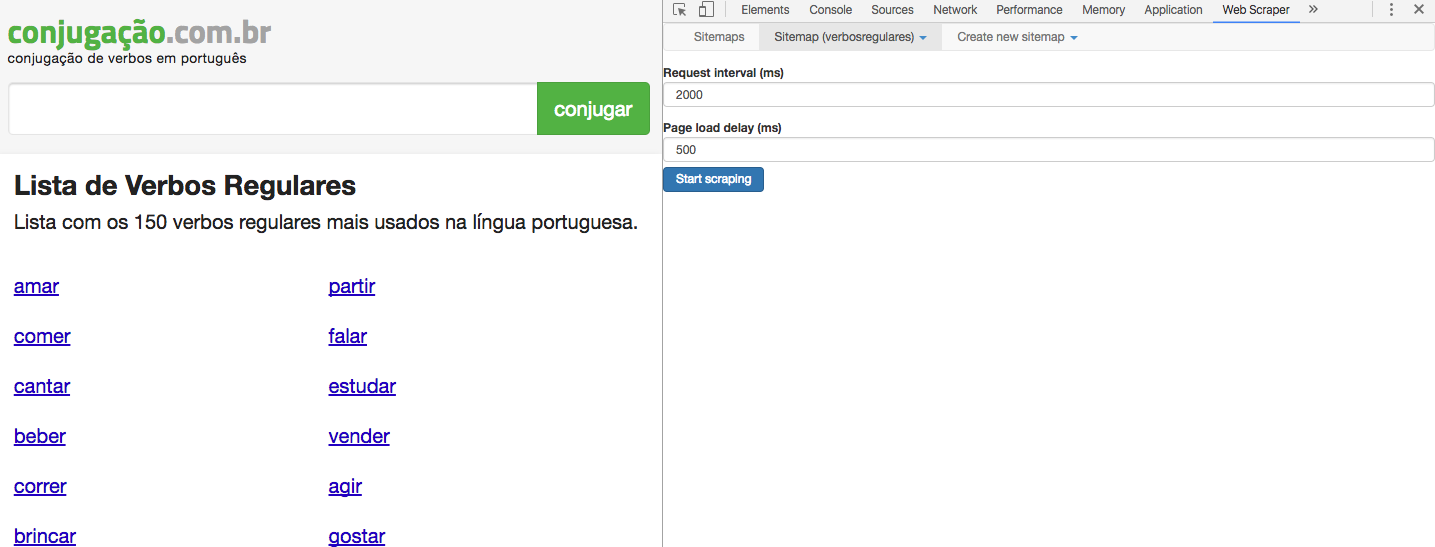
\includegraphics[width=\textwidth]{Screen_Shot_2017-10-05_at_22_54_20.png}
\end{frame}

%------------------------------------------------
\begin{frame}
\frametitle{Exemplo - Verbos}
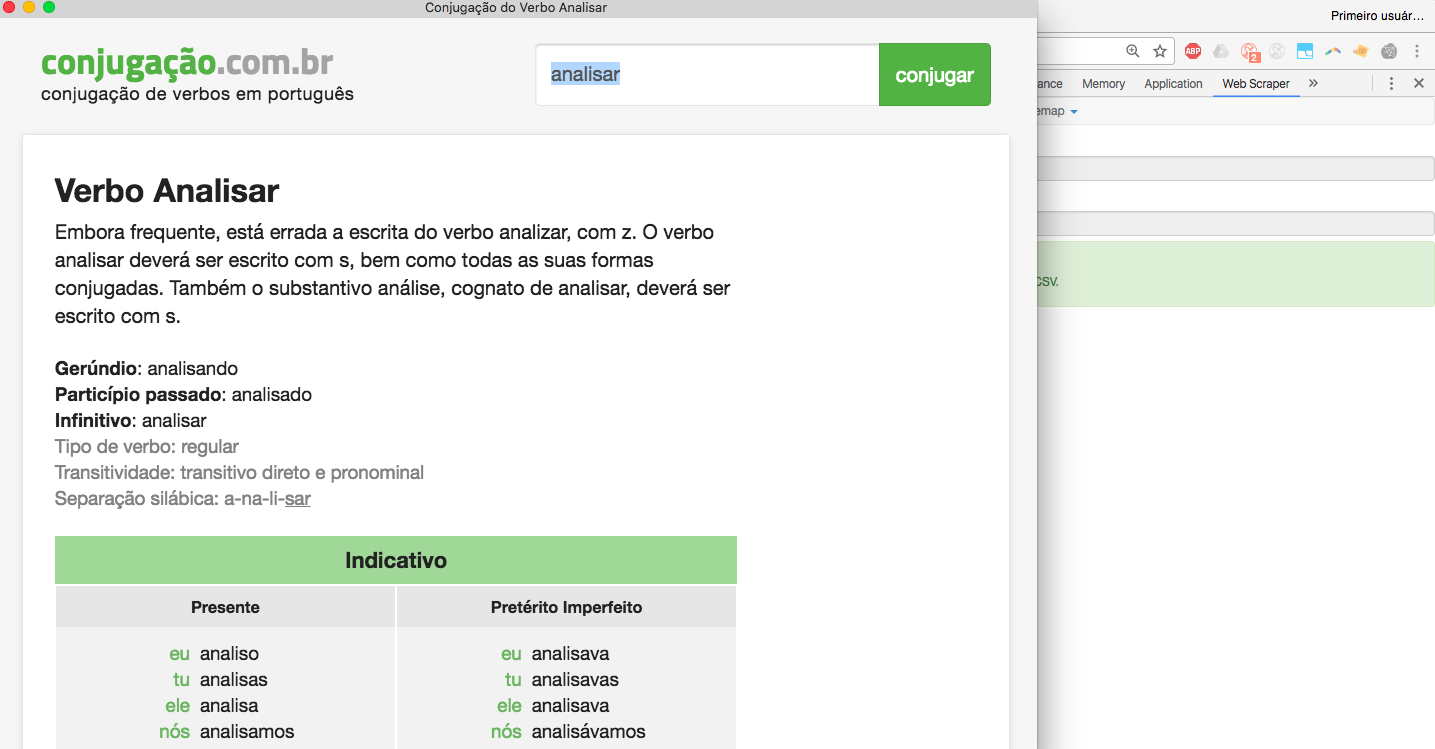
\includegraphics[width=\textwidth]{Screen_Shot_2017-10-05_at_22_56_54.png}
\end{frame}

%------------------------------------------------
\begin{frame}
\frametitle{Exemplo - Verbos}
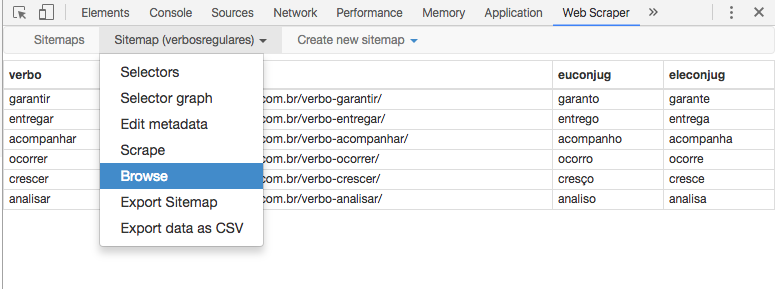
\includegraphics[width=\textwidth]{Screen_Shot_2017-10-05_at_22_57_15.png}
\end{frame}

%------------------------------------------------
\begin{frame}
\frametitle{Exemplo - Verbos}
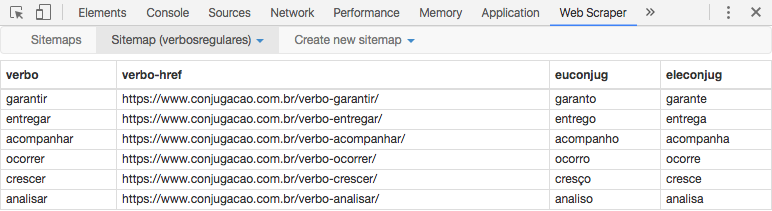
\includegraphics[width=\textwidth]{Screen_Shot_2017-10-05_at_22_57_22.png}
\end{frame}

\begin{frame}
\frametitle{Exemplo - Quadro Comparativo}
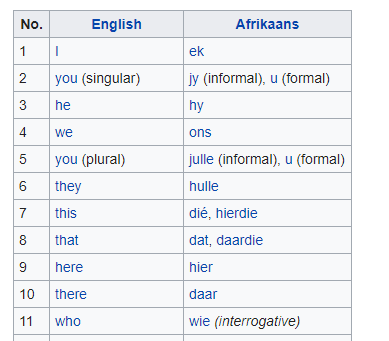
\includegraphics[width=\textwidth]{QuadroComparativo.png}
\end{frame}

\begin{frame}
\frametitle{Exemplo - Quadro Comparativo}
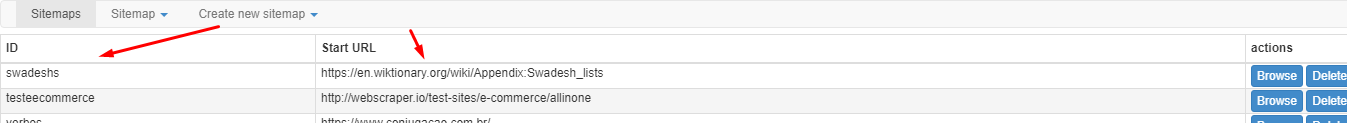
\includegraphics[width=\textwidth]{comparative1.png}
\end{frame}

\begin{frame}
\frametitle{Exemplo - Quadro Comparativo}
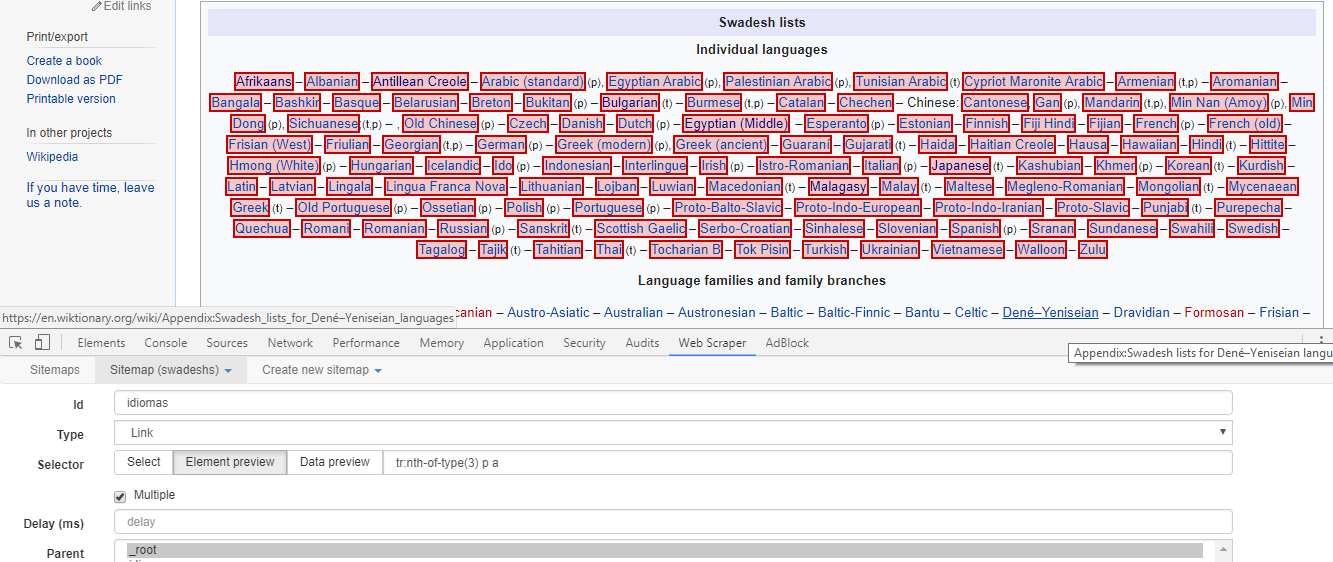
\includegraphics[width=\textwidth]{comparative2.png}
\end{frame}

\begin{frame}
\frametitle{Exemplo - Quadro Comparativo}
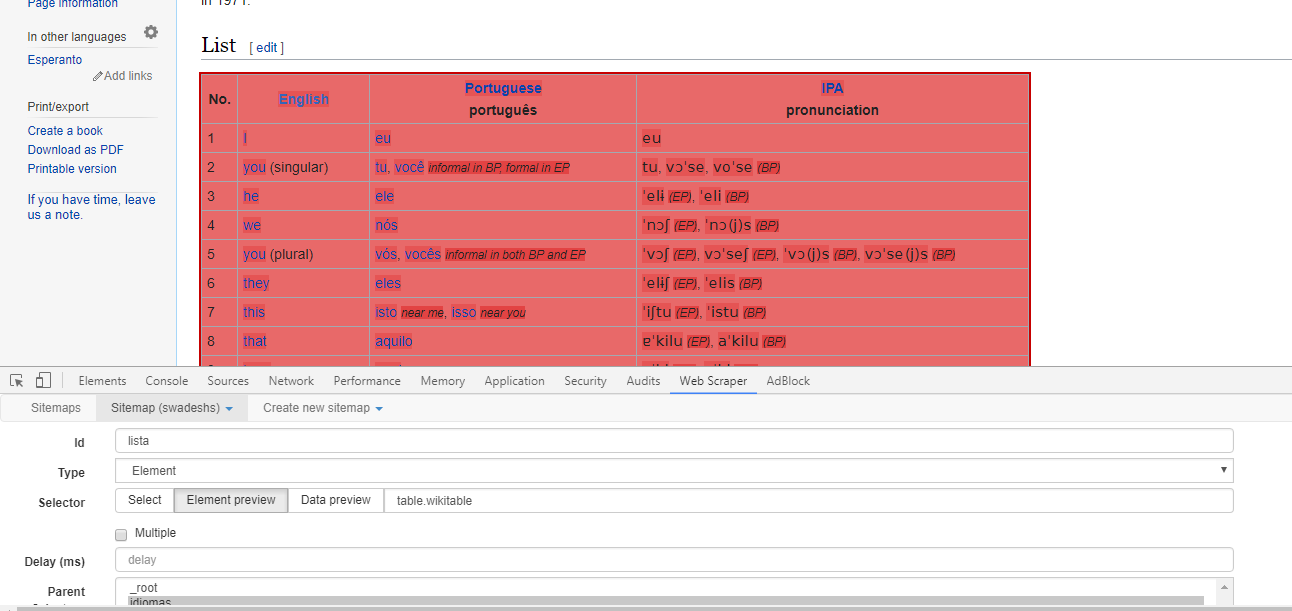
\includegraphics[width=\textwidth]{comparative3.png}
\end{frame}

\begin{frame}
\frametitle{Exemplo - Quadro Comparativo}
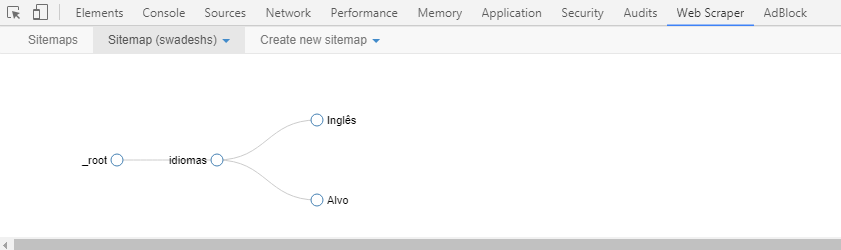
\includegraphics[width=\textwidth]{comparative4.png}
\end{frame}

\begin{frame}
\frametitle{Exemplo - Quadro Comparativo}
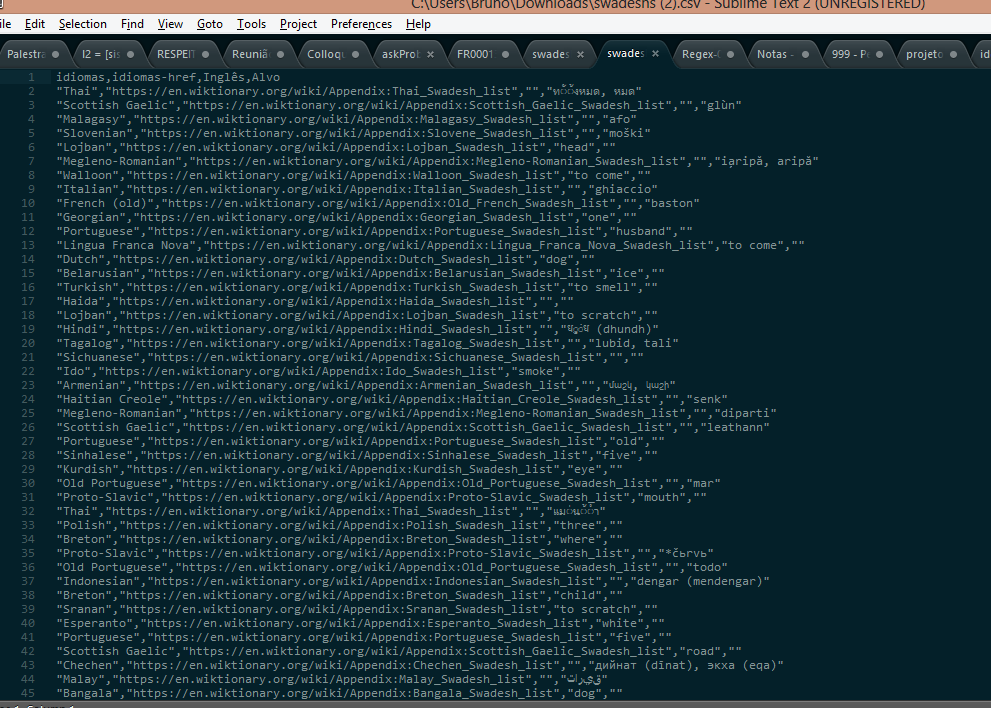
\includegraphics[width=\textwidth]{comparative5.png}
\end{frame}

\begin{frame}
\frametitle{Exemplo - Quadro Comparativo}
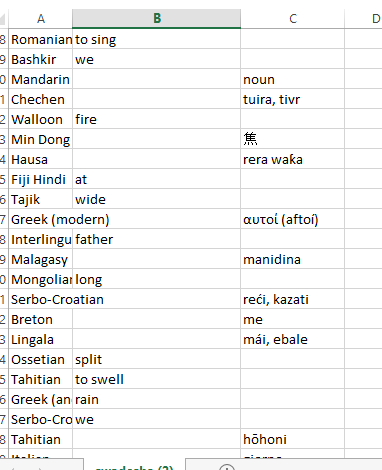
\includegraphics[width=\textwidth, height=\textheight]{comparative6.png}
\end{frame}

\begin{frame}
\frametitle{Exemplo - Palavras mais Buscadas}
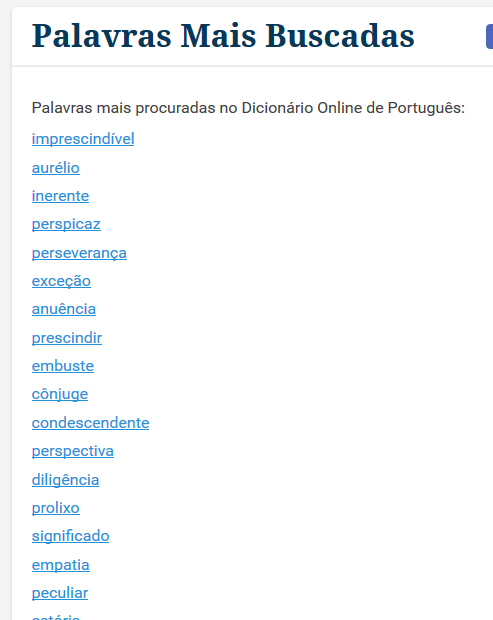
\includegraphics[width=\textwidth]{Dicio_com_br.png}
\end{frame}

\begin{frame}
\frametitle{Exemplo - Palavras mais Buscadas}
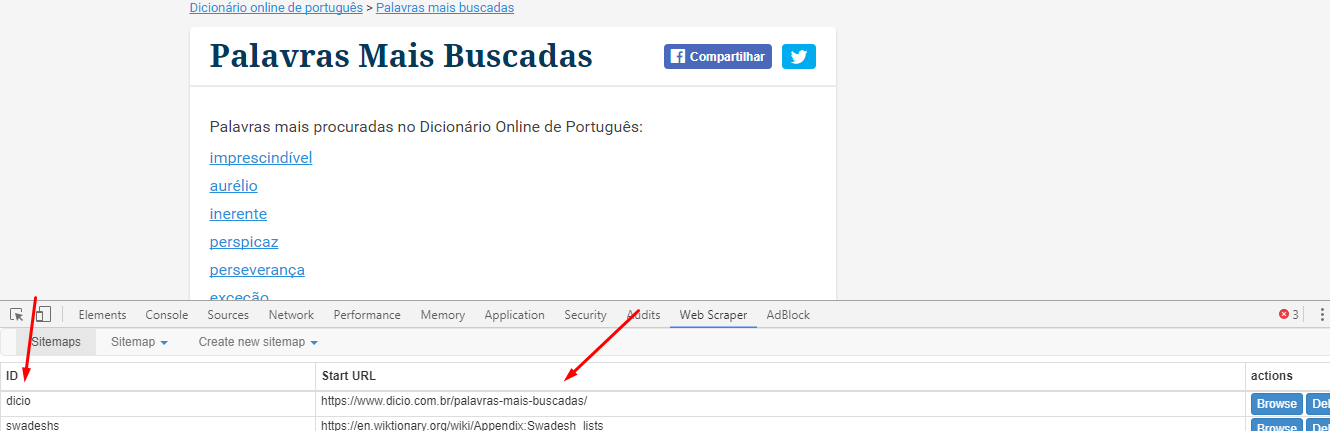
\includegraphics[width=\textwidth]{palavras_freq0.png}
\end{frame}


\begin{frame}
\frametitle{Exemplo - Palavras mais Buscadas}
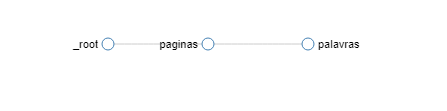
\includegraphics[width=\textwidth]{palavras_freq.png}
\end{frame}

\begin{frame}
\frametitle{Exemplo - Palavras mais Buscadas}
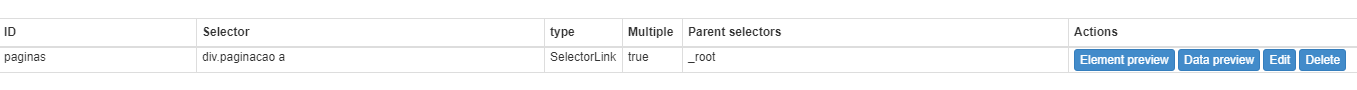
\includegraphics[width=\textwidth]{palavras_freq2.png}
\end{frame}

\begin{frame}
\frametitle{Exemplo - Palavras mais Buscadas}
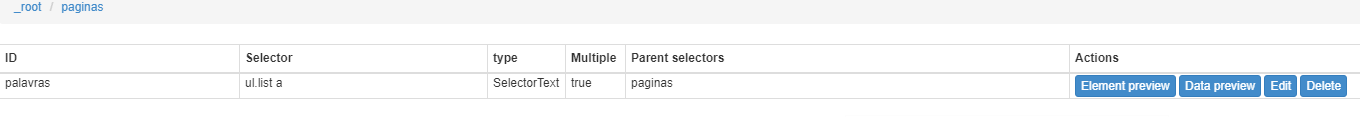
\includegraphics[width=\textwidth]{palavras_freq3.png}
\end{frame}

\begin{frame}
\frametitle{Exemplo - Palavras mais Buscadas}
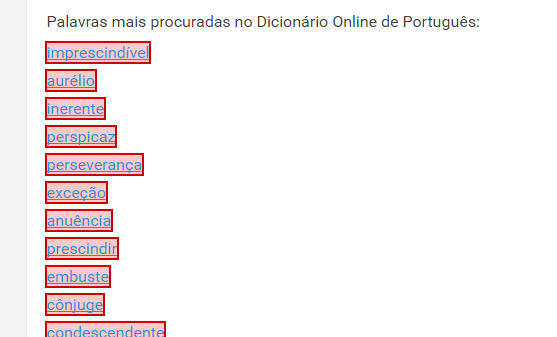
\includegraphics[width=\textwidth]{palavras_freq4.png}
\end{frame}


\begin{frame}
\frametitle{Exemplo - Palavras mais Buscadas}
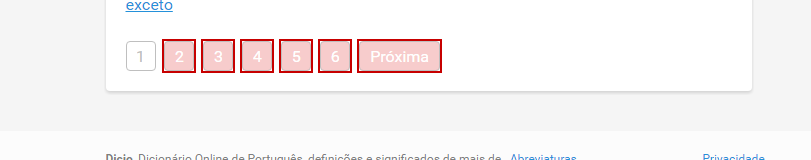
\includegraphics[width=\textwidth]{palavras_freq5.png}
\end{frame}


\begin{frame}
\frametitle{Exemplo - Palavras mais Buscadas}
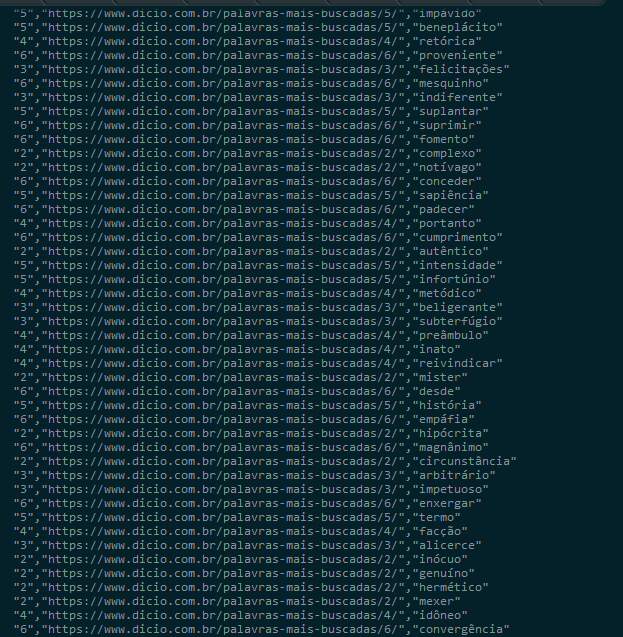
\includegraphics[width=\textwidth]{palavras_freq6.png}
\end{frame}

\begin{frame}
\centering{https://github.com/beatrizalbiero/presentations}
\end{frame}
\begin{frame}
\Huge{\centerline{Muito Obrigado!}}
\end{frame}


%----------------------------------------------------------------------------------------

\end{document}